 \subsection{Universidad de Mosku - Rusia}

\bigskip

\begin{tabular}{| l | c | c | c | c |}
 \hline 
Hop & IP &  RTT promedio (s)  & deltaRTT promedio & Ubicación\\
\hline 
1  &  192.168.0.1  &  0.00328697348541    &  0.00328697348541 & Argentina\\
\hline 
2  &  200.89.164.165  &  0.0182673031429    &  0.0149803296575 & Argentina\\
\hline 
3  &  200.89.165.130  &  0.018018808005    &  0 & Argentina\\
\hline 
4  &  200.89.165.222  &  0.023129620642   &  0.00511081263704 & Argentina\\
\hline 
5  &  206.165.31.213  &  0.0159362801966    &  0 & United States\\
\hline 
6  &  67.17.75.66  &  0.153266360362    &  0.137330080166 &  United States\\
\hline 
7  &  4.68.111.121  &  0.144784176125    &  0 & United States\\
\hline 
8  &  4.69.158.253  &  0.267091494686    &  0.122307318561 &  United States\\
\hline 
9  &  4.69.158.253  &  0.266443899045    &  0 & United States\\
\hline 
10  &  213.242.110.198  &  0.313186002227    &  0.0467421031829 & United Kingdom\\
\hline 
11  &  194.85.40.229  &  0.313147967716    &  0 & Russian Federation\\
\hline 
12  &  194.190.254.118  &  0.295875315396    &  0 & Russian Federation\\
\hline 
13  &  93.180.0.172  &  0.310500500249   &  0.0146251848526 & Moscow City Russian Federation\\
\hline 
14  &  188.44.33.30  &  0.293746012562    &  0 & Moscow City\\
\hline 
15  &  188.44.50.103  &  0.286035416261   &  0 & Moscow City\\
\hline 
\end{tabular}

\bigskip

\begin{figure}[H]
\centering
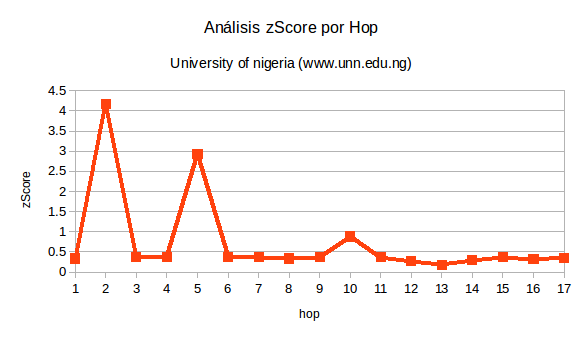
\includegraphics[width=1\textwidth]{graficos/RTT_rus.png}
\caption{RTT promedio por hop - Universidad de Mosku}
\label{Rus_rtt}
\end{figure}

\begin{figure}[H]
\centering
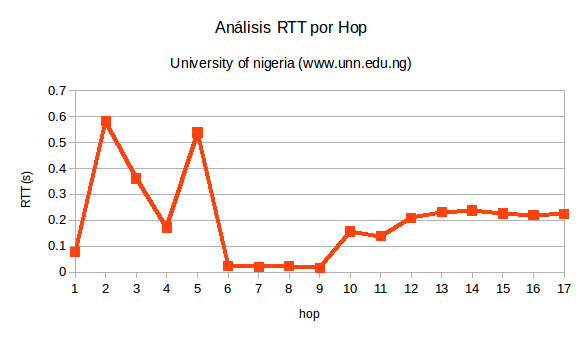
\includegraphics[width=1\textwidth]{graficos/zScore_rus.png}
\caption{zScore promedio por hop - Universidad de Mosku}
\label{Rus_zs}
\end{figure}
